\section{Extended Validation and Industrial-Resin Data}\label{app:completevalidation}
These studies add to the primary benchmark while retaining its original inputs
and results. The protocols record sampling units, source versions and numerical
failures. True diffusion locations and spectral amplitudes are reserved for
evaluation. The controlled TRAIn-MF study receives the generating factor count
to isolate optimization. Test acquisitions are excluded from fitting and
selection. The experimental studies state which
sample identities and diffusion references are supported by the source records.


\subsection{Controlled TRAIn-MF convergence and runtime curvature checks}\label{app:mfconvergence}
The supplementary study uses an isolated, instrumented copy of the regularized
MATLAB reference version 5.1, without substituting the later signed-data solver.
Nine synthetic matrices cross one, two and three finite-width shared profiles
with SNR 50, 100 and 200. Each contains 32 acquisitions and 24 signal-bearing
spectral channels with correlated amplitudes and overlapping peaks. The fitted
factor count is fixed to the generating count to isolate optimization; this
experiment does not validate automatic order selection. All 256 diffusion
nodes span $[0.1,15]\times10^{-9}\,\mathrm{m^2\,s^{-1}}$. The log-profile width is
$0.14$, with generating centers $(0.7,2.3,7.1)\times10^{-9}\,\mathrm{m^2\,s^{-1}}$
used in order as the factor count increases. The acquisition design is
$b_i=2.2\times10^9(i/31)^{1.7}$ for $i=0,\ldots,31$; every fourth row is reserved
for external prediction, leaving 24 fitting rows. Independent Gaussian noise
has $\sigma=1/\mathrm{SNR}$ after normalizing the maximum unattenuated signal to one.
The observations, two initialization seeds, penalties and tolerances are
held fixed across alternating warm-start caps of 1, 4, 8 and 16. Every arm has
the same subsequent 250-iteration SQP cap, with $\lambda_S=\lambda_A=10^{-8}$,
scaled KKT tolerance $10^{-6}$, objective tolerance $10^{-9}$, and inner-solver
tolerance $10^{-10}$ with a 2000-iteration cap. An early warm stop is permitted only
by the original objective-and-KKT rule. The configuration, seeds and inputs were
stored before inversion. A start already meeting the KKT rule may omit SQP,
as in the frozen reference. Numerical failures remain in the reported endpoints.

\begin{table}[htbp]\centering\small
\caption{Controlled warm-start comparison. Warm-only stationarity counts both
starts; final stationarity concerns the selected fit. CPU times are medians per
two-start fit, including instrumentation. The maximum final KKT and median clean
external prediction error include unconverged outputs.}
\begin{tabular}{rrrrrr}\toprule
Warm cap & Pre-SQP pass & Final pass & CPU (s) & Max KKT & RMSE/$\sigma$\\\midrule
1 & 0/18 & 3/9 & 152.0 & 4.67e-05 & 0.2740 \\
4 & 0/18 & 3/9 & 174.0 & 5.15e-05 & 0.2742 \\
8 & 0/18 & 4/9 & 214.1 & 4.23e-05 & 0.2737 \\
16 & 1/18 & 4/9 & 274.1 & 6.16e-05 & 0.2747 \\
\bottomrule\end{tabular}\end{table}

For the interior second-density-difference operator and $\lambda_S>0$ used
here, before every profile-block update and at each reported SQP iterate the revision checks
the conditional curvature criterion through $Kv\ne0$ and full row rank of $A$,
using the declared relative tolerance $10^{-10}$. If the criterion is numerically
unresolved before a profile update, that block uses an interior-point constrained
least-squares fallback with the same objective and constraints; the original
feasibility, descent and KKT checks still apply. No additional ridge, component
merging or chemical uniqueness claim is introduced. Numerical support at finitely
many checked iterates is not a uniform coercivity estimate or a convergence
certificate for the alternating/SQP procedure. Five targeted tests include
independent amplitude rows, duplicated rows, a constant kernel, zero amplitudes,
and an actual duplicated-row fallback. A separate warm-eight regression against
the uninstrumented frozen reference gives exactly equal predictions on the
declared rank-one check. These checks concern the new instrumented experiment,
not runtime checks retroactively attributed to the archived figure.

There is one realization per rank/SNR combination. This design examines
optimization within a fixed budget; it does not prove convergence of the factors
or identify physical constituents. Increasing the warm-start budget alone is
therefore insufficient evidence that the algorithm has converged.


Only 1/72 starts meet the KKT tolerance before SQP. After refinement, the selected
fits pass in 3/9, 3/9, 4/9, 4/9 cases for warm caps 1, 4, 8 and 16; 48/72 starts
reach the SQP iteration cap. SQP runs in 71/72 starts, with the remaining start
already satisfying the original KKT rule. On the nine paired inputs, predictions
from the warm-eight and warm-sixteen fits differ by a median 0.0018 and a maximum
0.0104 noise units on external rows. Their largest absolute relative objective
difference is 0.0295\%. These small differences show predictive stability on this
panel, but do not override the failed stationarity checks. Neither eight nor
sixteen warm sweeps guarantees a stationary final fit within the SQP budget.

The experiment records 14292 before-block/reported-SQP-iterate curvature checks, with 4 numerically unresolved conditions and 4 condition-triggered interior-point fallbacks. The final condition is supported for 72/72 starts. The targeted duplicate-row test exercises the fallback separately. Reevaluation of all 36 saved fits reproduces the stored pre-SQP/final objectives, KKT residuals and training-row predictions, checks common initializations and feasibility, and verifies monotonicity of saved objective histories at the original tolerance. This is a fresh-process audit of saved states, not a second execution of the optimizer or a reevaluation of every historical iterate. Runtime support and finite-budget stationarity are thus empirically different diagnostics. The four flagged checks arise in the same second initialization of the rank-three/SNR-200 input, once per warm cap; they are not four independent data realizations.

\begin{figure}[p]
\begin{adjustwidth}{-\extralength}{0cm}\centering
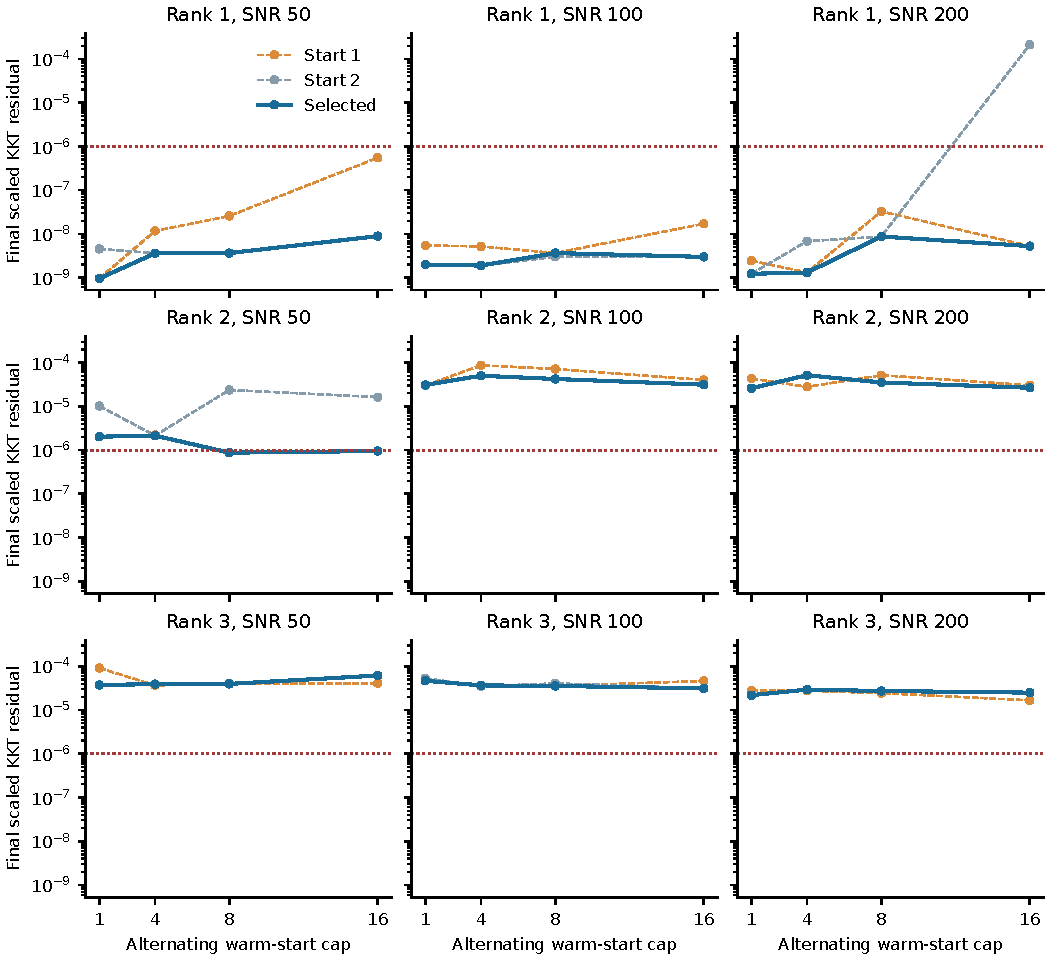
\includegraphics[width=\fulllength]{figures/mf_convergence_kkt.pdf}
\caption{Controlled TRAIn-MF warm-start sensitivity with a common subsequent
SQP budget. Numerical stationarity is assessed by the declared independent
KKT criterion; all unresolved outcomes are retained. Repeated budgets on
one rank/SNR input are paired conditions rather than new independent samples.}
\label{fig:mfconvergencerevision}
\end{adjustwidth}
\end{figure}


\subsection{Factorial separation of the shared selection stages}
\label{app:factorialcomplete}
% Draft fragment only; no manuscript sources modified.

We added a paired $2\times2$ intervention on the 36 signal-present atomic
problems, with a common proposal bank per method constructed from 18 fitting
rows, six reserved rows and the same final 24-row refit. $S=1$ forces the
conditional spectral mask and $S=0$ retains unrestricted amplitudes.
$P=0$ retains the native-selected nominal proposal order, whereas $P=1$
applies predictive order selection. Unsupported rates may disappear during
refinement, so the nominal proposal order is not necessarily the final active
order. The separate production reference permits both screened and unrestricted
candidates and reproduces the published selector; it is not a factorial cell.

\begin{table}[htbp]
\caption{Matched factorial experiment. Leakage and unmatched mass (UM) are
percentages. Recovery requires both order and log-rate matching.}
\label{tab:revision-factorial}
\centering
\begin{tabular}{llrrrrr}
\toprule
Path & Cell & Leakage & UM & $E_U$ & $W_{1,h}$ & Recovery \\
\midrule
RAI & $S0P0$ & 6.092 & 8.627 & 0.30677 & 0.16805 & 15/36 \\
RAI & $S1P0$ & 5.301 & 8.627 & 0.29087 & 0.15092 & 15/36 \\
RAI & $S0P1$ & 3.952 & 8.016 & 0.26189 & 0.14512 & 20/36 \\
RAI & $S1P1$ & 1.650 & 7.265 & 0.23145 & 0.10767 & 23/36 \\
DOME & $S0P0$ & 3.952 & 8.016 & 0.26189 & 0.14512 & 20/36 \\
DOME & $S1P0$ & 2.413 & 7.257 & 0.23856 & 0.11588 & 21/36 \\
DOME & $S0P1$ & 3.952 & 8.016 & 0.26189 & 0.14512 & 20/36 \\
DOME & $S1P1$ & 1.650 & 7.265 & 0.23145 & 0.10767 & 23/36 \\
Both & Production & 1.728 & 7.257 & 0.23299 & 0.10944 & 23/36 \\
\bottomrule
\end{tabular}
\end{table}

All 360 final outputs, including the separate production references, passed
their numerical checks; no selected candidate failed its numerical criterion.
The leakage interaction $(S1P1-S0P1)-(S1P0-S0P0)$ is $-1.511$ percentage
points for RAI (paired problem-bootstrap 95\% interval $[-2.603,-0.598]$)
and $-0.763$ for DOME ($[-1.670,-0.186]$). These descriptive intervals do
not establish a universal interaction or provide multiplicity-adjusted inference.
The two final proposal paths remain effectively equivalent. DOME's unmatched
mass increases slightly from $S1P0$ to $S1P1$ despite lower average leakage and
prediction error. Original signal masks are retained, including their original
internal-validation reuse; this is a matched mechanism comparison, not a new
calibration experiment. Per-arm logical cost accounts for shared candidate
fits and does not represent separately measured end-to-end timing.
In the weak-component problem \texttt{test\_011\_weak}, forced screening and
prediction return three rates but match only two true rates; the minority rate
remains unrecovered. Its lower $E_U$ and $W_{1,h}$ therefore do not establish
recovery of the additional species. Correct order rises from 25 to 26 problems
relative to production choice, while complete recovery remains 23/36 for both.


\subsection{Adaptive weak-component recovery}\label{app:weakpower}
Ninety-six new problems span four generating minority-amplitude factors: 0.02, 0.04, 0.08 and 0.16. Three SNRs (50, 100 and 200), with eight independent truth/noise realizations per cell, complete the design. Each factor multiplies the third spectral
template before the total unattenuated signal is normalized; it is not a
molar fraction. The mask is formed from fitting acquisitions only, excluding
both internal validation and external test rows. The frozen adaptive selector
and rate-matching tolerance remain unchanged.

\begin{figure}[p]
\begin{adjustwidth}{-\extralength}{0cm}\centering
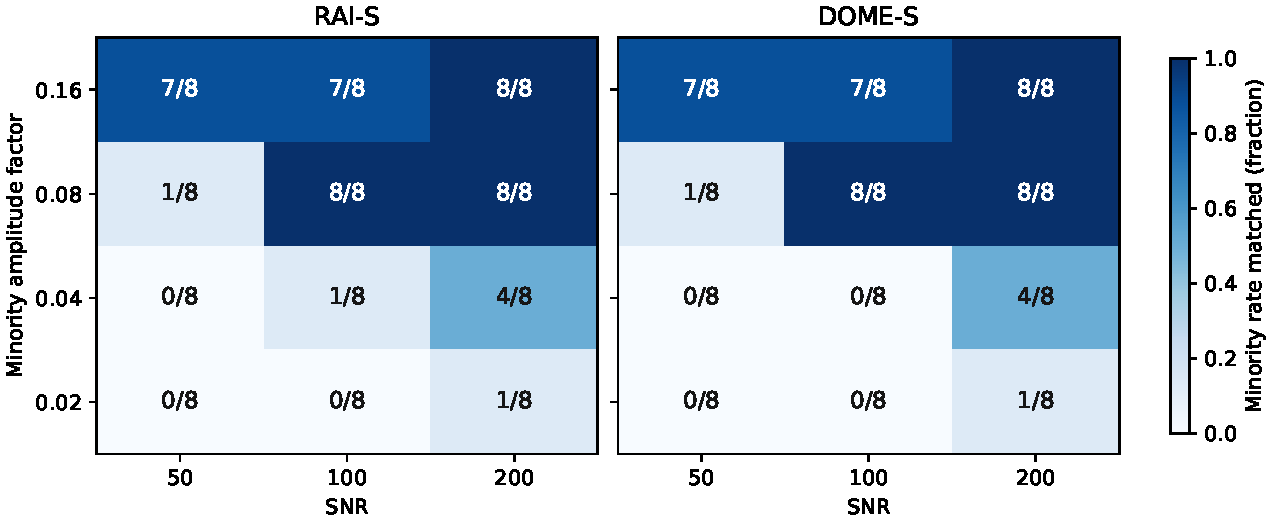
\includegraphics[width=\fulllength]{figures/weak_power_revision.pdf}
\caption{New weak-component panel. Each cell counts matched minority rates in
eight independent problems, using the original log-rate tolerance 0.25.
The methods use paired inputs. These counts estimate recovery under the
declared generator, not a calibrated probability of chemical presence.}
\label{fig:weakpowerrevision}\end{adjustwidth}
\end{figure}

All 192 method fits pass their numerical criteria. RAI-S matches the minority
rate in 45 of 96 problems and DOME-S in 44 of 96; these are paired method
results, not 192 independent chemical mixtures. At factor 0.02 the counts
across increasing SNR are $(0,0,1)/8$ for both methods. At factor 0.08 they
are $(1,8,8)/8$. The intermediate factor 0.04 gives $(0,1,4)/8$ for RAI-S
and $(0,0,4)/8$ for DOME-S. These visible failures prevent a general claim
of reliable weak-component discovery. Masking also contributes: mean retained
minority spectral mass varies from about 0.59 at the weakest low-SNR cell to
0.99 at the strongest high-SNR cell. A channel outside the mask is unestimated.

Exact two-sided 95\% Clopper--Pearson intervals are retained per cell in the
machine-readable supplement; for example, zero of eight gives an upper
endpoint 0.369 and eight of eight a lower endpoint 0.631. They are descriptive
cell-wise intervals without multiplicity adjustment. Aggregate counts across
the prespecified SNR/factor mixture are not a universal power guarantee.


\subsection{Expanded neural policy evaluation}
% Numerical values originate from the preserved final_summary.json.

\label{app:neuralexpanded}
We trained five CPU networks with different seeds using the same 80-problem
trace bank. Each run separates 64 training from 16 validation problems and uses
training records alone to normalize features. Checkpoint replay is exact.
The new test panel contains 120 problems: 72 in the original physical domain,
24 at unseen SNRs (25, 35 and 500), and 24 with unseen acquisition exponents
and diffusion weightings. The five policies and the deterministic proposal-order
control share the six-round cap, a shortlist of one with fallback, and the same
numerical verifier. The control is the classical shortlist variant; it differs
from both the exhaustive controller and the atomic RAI estimator.
\begin{table}[htbp]
\caption{Independent neural evaluation. $W_{1,h}$ averages 105 signal-present problems; $E_U$ includes all 120 problems, including 15 null controls. Numerical success is a solver criterion. Times are mean solver seconds and exclude checkpoint loading and serialization.}
\label{tab:neuralexpanded}
\centering
\begin{tabular}{lrrrrr}
\toprule
Method & $W_{1,h}$ & $E_U$ & Numerical success & Seconds & Tree fits \\
\midrule
Classical shortlist & 0.33383 & 0.29961 & 120/120 & 22.03 & 20.76 \\
RAI-Net 172901 & 0.33341 & 0.29956 & 120/120 & 17.44 & 19.24 \\
RAI-Net 172902 & 0.33319 & 0.29941 & 120/120 & 18.91 & 19.66 \\
RAI-Net 172903 & 0.33323 & 0.29952 & 120/120 & 18.13 & 19.49 \\
RAI-Net 172904 & 0.33390 & 0.29951 & 120/120 & 18.87 & 18.94 \\
RAI-Net 172905 & 0.33271 & 0.29944 & 120/120 & 19.15 & 19.55 \\
\bottomrule
\end{tabular}
\end{table}

The seed-average neural-minus-classical $W_{1,h}$ difference is $-0.00054$ (paired problem-bootstrap 95\% interval $[-0.00174, 0.00056]$); the corresponding $E_U$ difference is $-0.00012$ ($[-0.00044, 0.00010]$). The pooled bootstrap resamples whole problems within each domain, preserving domain counts; the five seed outputs on a problem are paired, not independent tests. Individual seed mean $W_{1,h}$ differences range from $-0.00111$ to $0.00007$.
ID: $\Delta W_1=-0.00136$, interval $[-0.00294, -0.00003]$ ($n=63$); individual seed differences range from $-0.00165$ to $-0.00076$. OOD\_noise: $\Delta W_1=-0.00059$, interval $[-0.00230, 0.00070]$ ($n=21$); individual seed differences range from $-0.00142$ to $0.00013$. OOD\_acquisition: $\Delta W_1=0.00197$, interval $[-0.00135, 0.00559]$ ($n=21$); individual seed differences range from $-0.00106$ to $0.00430$.
All 720 final method outputs pass their numerical checks, with 0 execution errors
and 0 failed final checks. The analysis retains failed numerical outputs whenever
they occur, rather than removing them from the averages.
Intermediate failures still occur: 98/2371 control subproblems and 476/11026 neural
subproblems fail the search-stage checks, with 91--99 failures per policy. Each
method encounters at least one failed search fit in 48/120 problems. The selected
training paths and all final refits nevertheless pass their checks. These counts
describe solver events and should not be treated as independent statistical trials.
Mean differences from the classical control are $-3.524$ seconds per problem
for solver time and $-1.382$ for the number of fixed-tree fits (neural minus
classical). Equal search caps therefore do not imply equal realized effort.
The five network fits and checkpoint writes take 3.455 seconds after data loading
and the Torch import. The reused traces record 1690.7 seconds of summed historical
generation time, which is a different quantity from wall time for this revision.
These measurements do not establish an end-to-end speedup. Four selected
checkpoints reach the 400-epoch budget, so learning convergence is also unresolved.
The study supports neither a universal accuracy advantage nor experimental
chemical identification.

An exploratory breakdown by problem family finds lower mean shape error for
all five policies on the 15 broad-profile problems, but higher error for four
of the five policies on the 90 atomic problems. We did not use these patterns
to select a seed or tune the models. They are post-hoc observations, not
independent confirmatory tests.

\begin{figure}[p]
\begin{adjustwidth}{-\extralength}{0cm}\centering
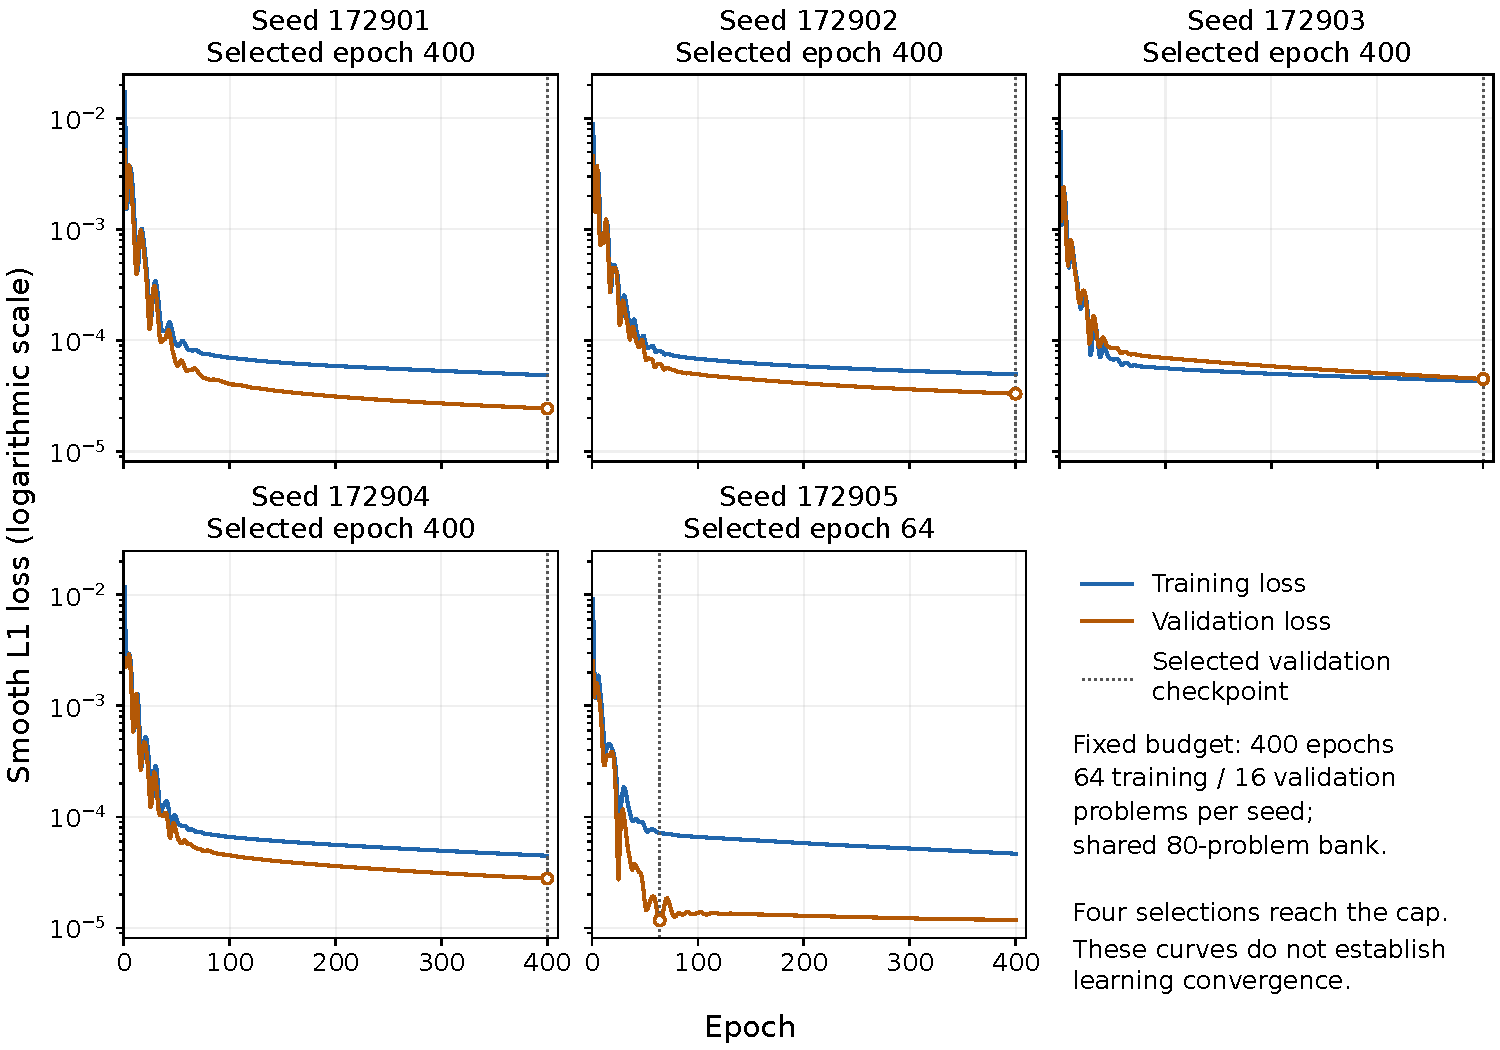
\includegraphics[width=\fulllength]{figures/neural_learning_curves.pdf}
\caption{Training and whole-problem validation Smooth L1 loss for five separately
seeded RAI-Net rankers. Each run uses 64 training and 16 validation problems
from the same historical 80-problem bank. Dotted lines and open markers
identify the lowest observed validation-loss checkpoint. Four selections
reach the declared 400-epoch budget, so these histories do not establish
learning convergence. The historical trainer records training loss before
the Adam update and validation loss after it. Test observations are absent from normalization,
training and checkpoint selection.}\label{fig:neurallearning}
\end{adjustwidth}
\end{figure}


\subsection{Shared external-reference comparison}\label{app:externalcomparison}
The additional comparison uses the same frozen observations, masks and outer
test acquisitions. The physical interval is common to grid methods and
positive-measure eligibility. Native continuous fits are retained with their
original rate constraints rather than silently projected into that interval. Matrix
zero served as an adapter pilot and is retained in the raw outputs but excluded
symmetrically from the iid summary, leaving 47 matrices (41 signal-present and
six null). Twelve underlying signal-present problems also receive each of the
baseline and correlated-noise stresses. These are retrospective comparisons,
not a new untouched synthetic population. Outer test rows are not used in
the internal parameter or order decisions.

SCORE uses the attributed GNAT translation, signed conditional least squares
and its original initialization, with a declared reserved-acquisition wrapper
selecting orders zero through four. Candidate selection enforces interval
eligibility, but the final continuous refit is unconstrained in log rate;
out-of-interval results are retained and flagged. The positive-amplitude
sensitivity uses the same wrapper and proposal budget. LOCODOSY retains its native local SVD
order and reduction rules on the common contiguous signal windows; its sum of
local components is not a global molecular count. Its native rate domain has
zero as the lower limit and the common upper limit. LOCODOSY uses the training
observations for its order rule; only the validation-selected adapters use
the internal split. Five of the 47 iid LOCODOSY outputs contain rates outside
the declared positive-measure interval; none is projected or discarded.
No outer test row participates in these decisions. Positive Tikhonov selects
its curvature weight from $\{0.01,1,100,10^4\}$ on internal validation.
The PALMA constrained objective uses a training-only positive low-$b$ scale,
entropy weights $\{0.01,0.1,0.5\}$ selected on internal validation, a declared
95\% Gaussian noise-ball radius and 5000 final PPXA+ iterations. A batched
Woodbury graph projection was checked against the reviewed scalar QR engine;
this is an implementation of the stated objective, not a claim of identical
performance to all upstream application presets.

\begin{table}[htbp]\centering\small
\caption{Common external-reference comparison. $E_U$ is clean external error
in noise units over signal-present cases. Numerical success uses each method's
own criterion; all returned outputs enter $E_U$, including nonconverged ones.
The denominator after $W_{1,h}$ counts only outputs admitting a nonnegative
measure within the declared interval and is therefore a different population
for signed methods.}\label{tab:externalexecuted}
\begin{tabularx}{\linewidth}{@{}Xrrr@{}}\toprule
Method & Numerical success & $E_U$ & $W_{1,h}$ [n]\\\midrule
RAI-S & 47/47 & 0.23477 & 0.1201 [41]\\
DOME-S & 47/47 & 0.23477 & 0.1201 [41]\\
SCORE-CV (signed) & 47/47 & 0.30329 & 0.0000 [3]\\
SCORE-NNLS-CV & 47/47 & 0.26681 & 0.1563 [41]\\
LOCODOSY (signed) & 47/47 & 0.26114 & 0.0013 [4]\\
Positive Tikhonov & 47/47 & 0.33523 & 0.3057 [41]\\
PALMA objective + CV & 0/47 & 0.73627 & 0.4225 [41]\\
\bottomrule\end{tabularx}\end{table}

The table compares prediction under the stated fitting conditions, rather than
chemical identification. Signed cancellation can reduce error without yielding
a positive component representation. Similarly, PPXA+ has not reached the required
optimality criterion for the PALMA objective, so its finite-budget result cannot
rank the fully optimized method. The supplement retains all convergence flags
and curve-level constraint diagnostics. CONTIN, UPEN, DRECT and DREAM were not
run under this common protocol; Table~\ref{tab:externalmethods} states what those
comparisons would require. Positive Tikhonov is a separate control and is not
presented as the full CONTIN procedure. The executed comparisons cover the
closest joint-component references and two positive distributional controls.

On the twelve baseline-stress cases, positive SCORE has a slightly smaller
mean clean error than RAI-S ($1.00044$ versus $1.01092$ noise units); the
paired descriptive interval for the difference is $[-0.02583,0.00196]$ and
includes zero. There is no demonstrated robust advantage on this offset
panel. Correlated-noise results and all paired contrasts are included in
the machine-readable supplement; they are not independent replications of
the underlying twelve signal configurations.


\subsection{Experimental prediction on industrial resin spectra}\label{app:experimentalrevision}
We analysed spectra from four industrial-resin specimens in the TP194 series 2623086, 2623088,
2623084 and 2619082. Each series contains three blocks at diffusion times 75, 100
and 125~ms, with 23 acquisitions and 65,536 spectral channels per block. The twelve
blocks belong to four specimens and are not independent mixture preparations.
We fit all 17,386--21,314 channels per block within the detected positive absorption
support, preserving their measured signs. Five acquisitions are withheld for
prediction, and support detection also excludes the internal validation rows.
A single scalar normalizes each matrix; channels are neither rescaled individually
nor replaced by integrated bands or a thinned fit grid. Outside the support,
signal remains unestimated. The full-spectrum check detects 75--219 strongly
negative points per block, including 53--187 outside the positive support.
We apply no automatic phase, baseline, absolute-value or clipping correction.

RAI-S and DOME-S use their frozen support-aware estimators with a four-atom search cap. SCORE-CV uses the attributed SCORE implementation with signed amplitudes and native initialization, augmented by internal acquisition-based order selection over one to four atoms~\cite{score}. SCORE-NNLS-CV changes the conditional amplitude problem to NNLS while retaining the same initialization, optimizer budget and selection wrapper; it is explicitly a constrained variant, not the original signed SCORE method. LOCODOSY-SCORE retains the native local singular-value order heuristic and reduction rules~\cite{locodosy}, using the same detected windows. Its output rows are local contributions, not a global species count. Small-rank batched NNLS is checked against the native per-channel solver; the RAI objective, gradient and predictions are also checked against the original implementation. All selected channels contribute to every reported error.

\begin{table}[htbp]
\caption{Experimental acquisition-holdout prediction on twelve blocks, grouped into four industrial resin specimens. NRMSE divides held-out RMSE by the training RMS on the same support. NC counts final global optimizer nonconvergence; unstable flags denote kernel condition above $10^8$ or amplitude expansion above $10^4$; cap counts selection of the maximum four global atoms. These flags are not exclusions. Dashes denote quantities that are not global estimands for LOCODOSY.}\label{tab:experimentalrevision}
\centering\small
\begin{tabular}{lrrrrr}\toprule
Method & Mean NRMSE (\%) & Median (\%) & NC & Unstable & Cap\\\midrule
RAI-S & 1.1226 & 1.1119 & 0 & 0 & 12\\
DOME-S & 1.1226 & 1.1119 & 0 & 0 & 12\\
SCORE-CV & 0.7740 & 0.7884 & 6 & 8 & 8\\
SCORE-NNLS-CV & 1.1230 & 1.1119 & 0 & 0 & 12\\
LOCODOSY-SCORE & 0.8914 & 0.8620 & -- & -- & --\\
\bottomrule\end{tabular}
\end{table}

All 60 of 60 planned predictions were completed. RAI-S and DOME-S reach the cap
and trigger the atomic-model mismatch warning in all twelve blocks. Their largest
relative prediction difference is $1.41\times10^{-12}$, providing no independent
predictive advantage for either proposal mechanism. Reaching the cap also does
not establish four chemical species. Positive SCORE serves as a constraint
control. Signed SCORE predicts better in several blocks, but 6 of its twelve
final fits fail to converge within the budget and 8 have unstable global
amplitudes. We retain these predictions in the table. LOCODOSY covers 174 windows,
with 0 nonconverged local fits and 0 failed windows. Low prediction error from
cancelling signed amplitudes alone cannot establish reliable identification.


Background neighbouring-channel correlations range from 0.999198 to 0.999757. Consequently, the background MAD scale is descriptive, and these processed data do not validate an independent-Gaussian interpretation of support scores or channel-wise confidence intervals. Acquisition-order effects and residual phase/baseline distortion are not separately identified. Spectral-factor matching across the three diffusion times is reported as a descriptive consistency check, not as chemically verified correspondence.

The original HDO/TBO calibration is retained, with 1,932 experimental source hashes, 115 HDO reference source hashes and twelve saved-input hashes rechecked. If $D=10^{-9}c\kappa$, where $c$ is the calibration coefficient, first-order uncertainty propagation would require
\begin{equation}
 \operatorname{Var}(D)\simeq 10^{-18}\left[\kappa^2\operatorname{Var}(c)+c^2\operatorname{Var}(\kappa)+2c\kappa\operatorname{Cov}(c,\kappa)\right].
\end{equation}
The reference and thermal-model contributions to $\operatorname{Var}(c)$ are not quantified in the source calibration; they are not set to zero. The maps are conditional on that calibration, and no absolute diffusion-accuracy interval or molecular-weight estimate is asserted.

The available records do not link these four identifiers to a verified composition.
We therefore assign no compositions or diffusion values from other batches to
these specimens. The measurements provide evidence about prediction on industrial
resins, but not a test against known component counts or independently measured
component diffusion coefficients. This is especially relevant when finite atomic
models are fitted to potentially polydisperse materials.

\begin{figure}[p]
\begin{adjustwidth}{-\extralength}{0cm}
\centering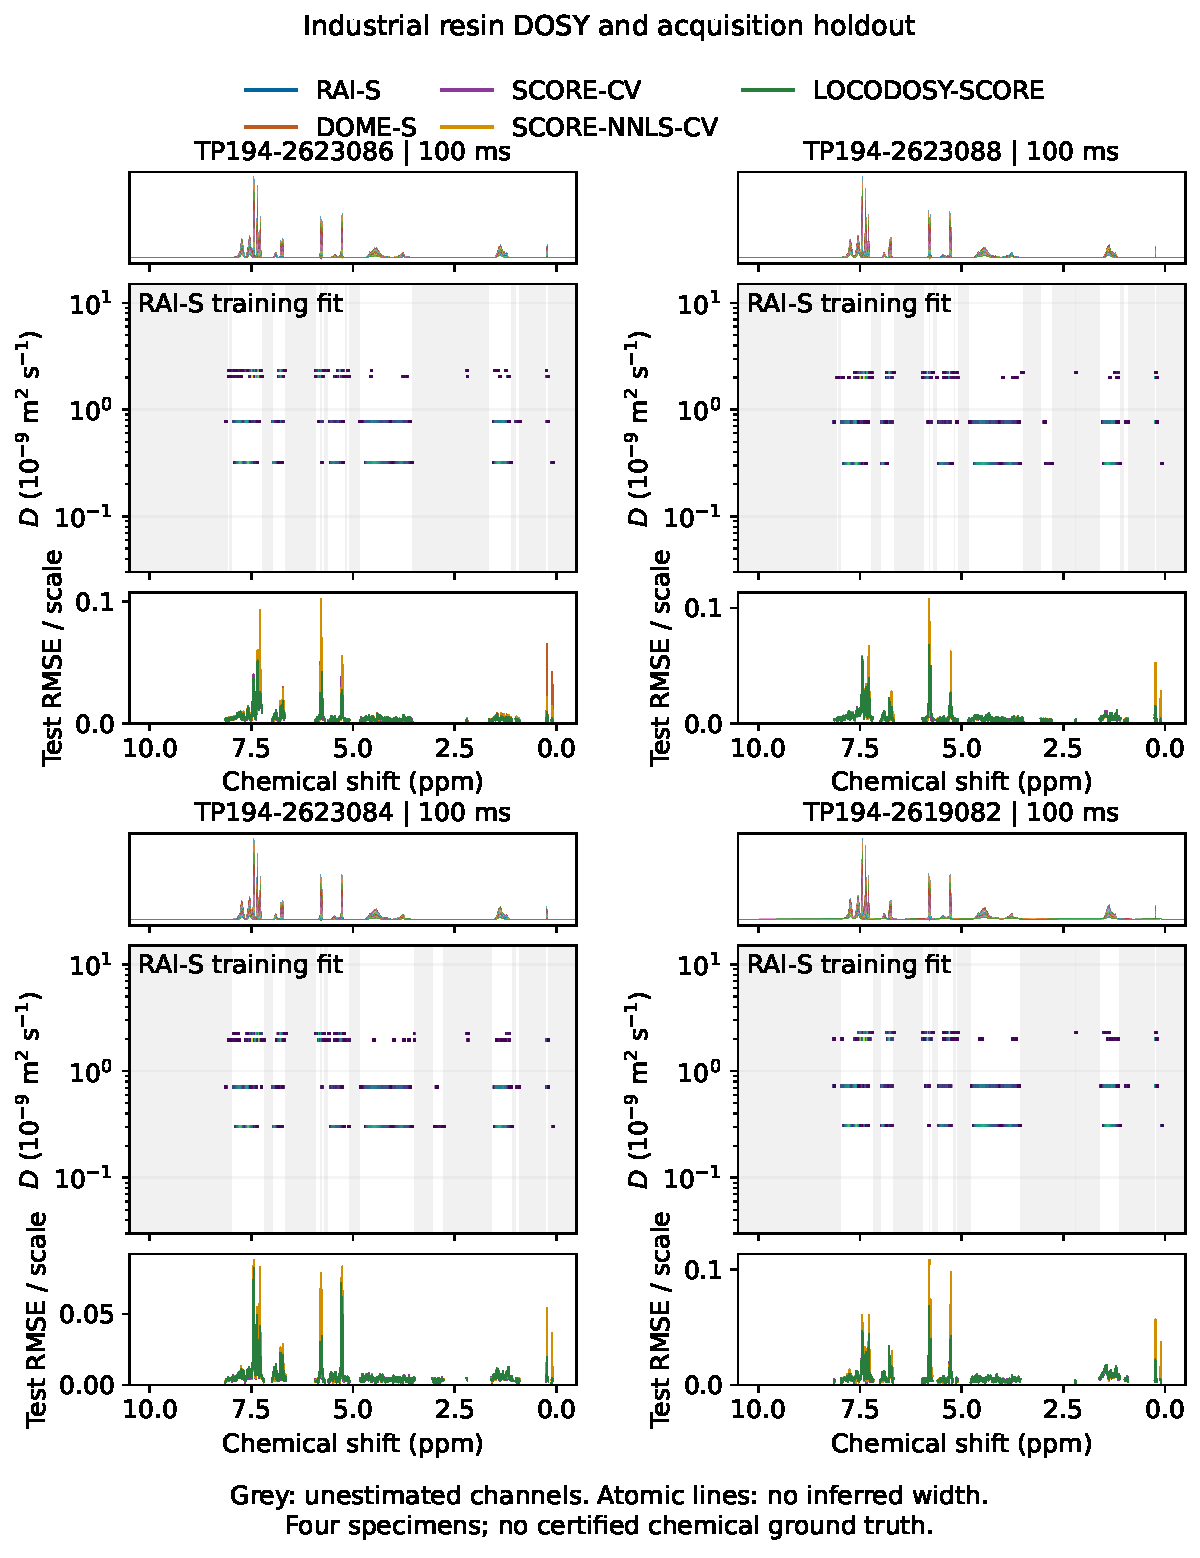
\includegraphics[width=\fulllength,height=0.86\textheight,keepaspectratio]{figures/experimental_four_series.pdf}
\caption{Industrial resin spectra at 100~ms: measured spectral families (top), RAI-S training-fit atomic DOSY maps (middle) and held-out error profiles for the five estimators (bottom). All detected support channels enter the fits; grey map regions are unestimated. Display thinning is confined to traces and error curves. Atoms are shown without fabricated distributional widths, and no chemical ground-truth map is available.}\label{fig:experimentalresins}
\end{adjustwidth}
\end{figure}
\begin{figure}[p]
\begin{adjustwidth}{-\extralength}{0cm}
\centering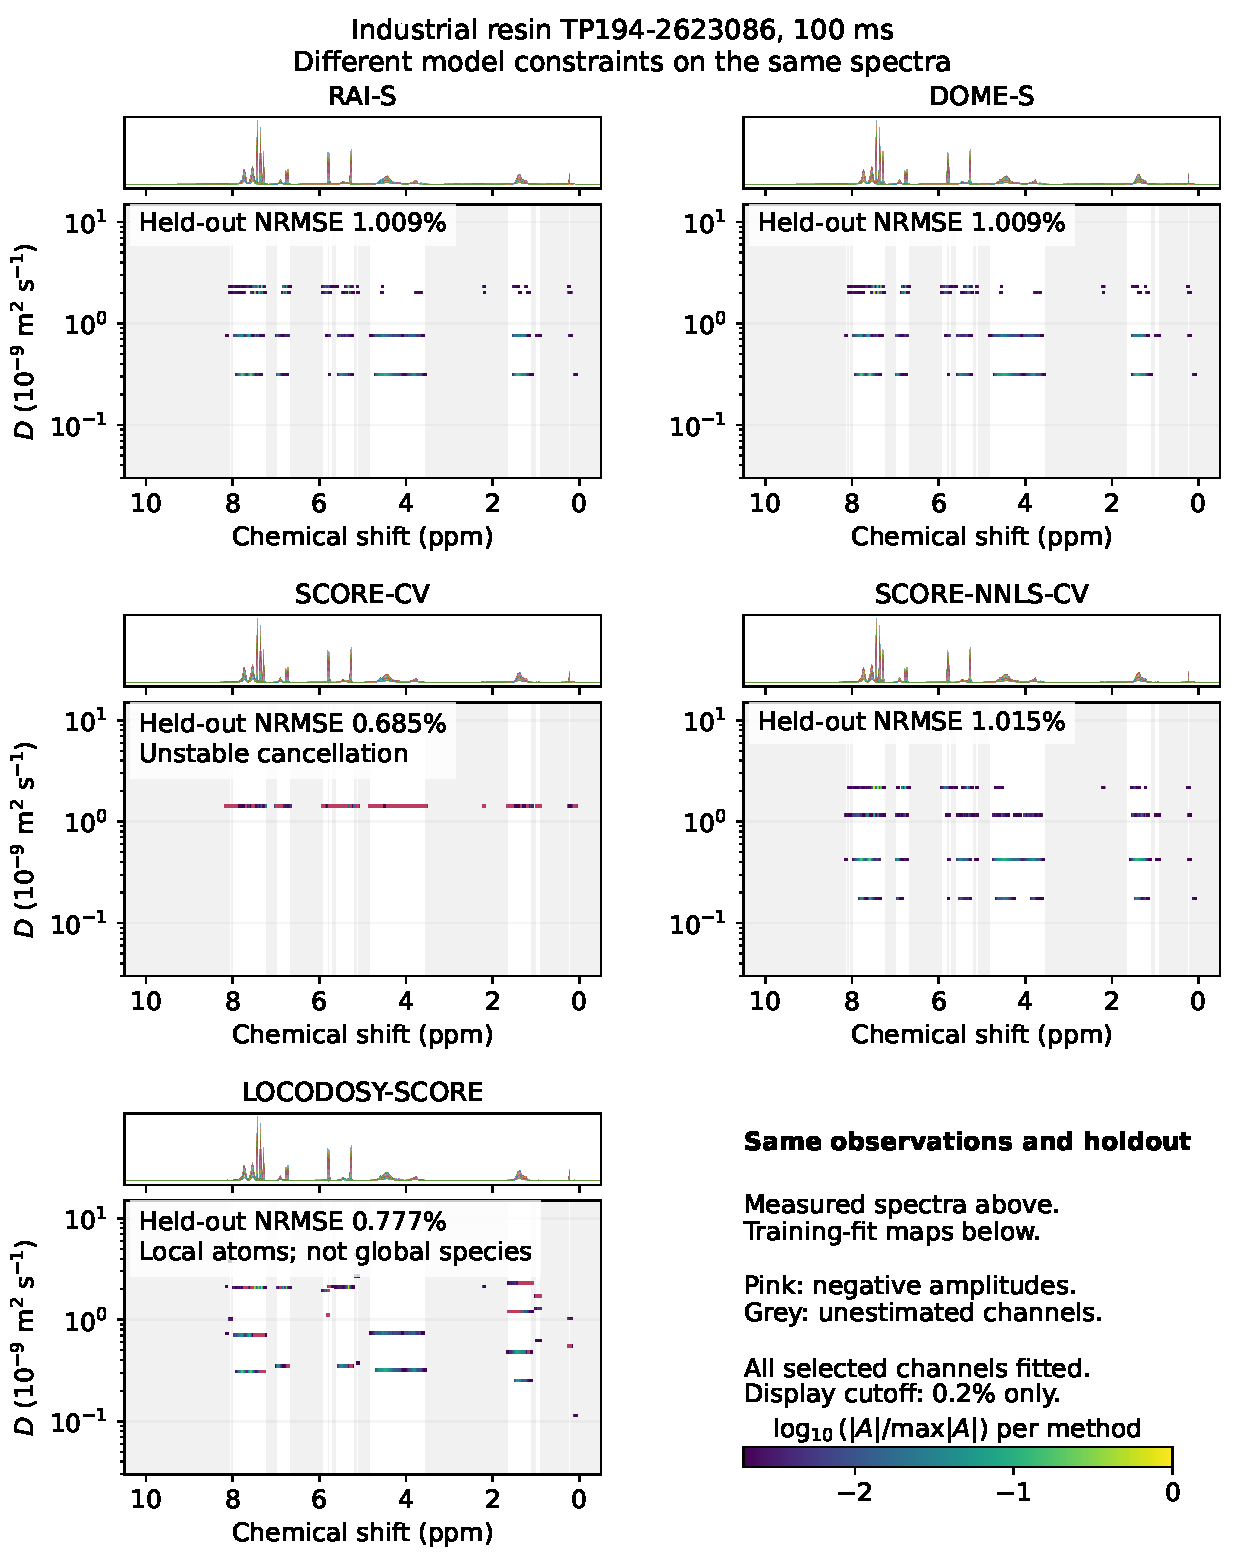
\includegraphics[width=\fulllength,height=0.86\textheight,keepaspectratio]{figures/experimental_methods_T1_B2.pdf}
\caption{The five estimators on industrial resin TP194-2623086 at 100~ms, using identical observations and acquisition holdout. Colours show relative absolute amplitude within each method; negative amplitudes are pink and unestimated regions are grey. The 0.2\% display cutoff does not affect fitting or scoring. The nearly coincident signed SCORE atoms exhibit large cancellation despite a lower held-out prediction error. LOCODOSY lines are local contributions.}\label{fig:experimentalmethods}
\end{adjustwidth}
\end{figure}


\subsection{A public multicomponent DOSY example}\label{app:publicmixture}
We additionally processed the public \texttt{PropPentSuc\_DOSY.fid} example
distributed by the official DOSY Toolbox downloads page\cite{dosytoolboxdata}.
Its internal sample text documents propanol and sucrose in D$_2$O; its directory
name is consistent with the 1-propanol/1-pentanol/sucrose example illustrated
in the GNAT manual\cite{gnatmanual}. The latter does not explicitly identify
this archived file, so pentanol is not treated as a verified additional label.
Neither a certified complete composition nor independently measured diffusion
coefficients accompany the example used here. It therefore supplies a public
multicomponent experimental check, not known-order or absolute-$D$ ground truth.

The archive contains 30 acquired gradient levels. Acquisitions
4, 8, 12, 16, 20, 24 and 28 were reserved for external prediction;
five of the remaining acquisitions formed the internal validation split.
A single common linear ACME phase\cite{acme} was estimated from the other
18 discovery acquisitions after Fourier transformation and then frozen for
all methods and acquisitions. The archived phase alone had left visible
dispersion in discovery-only quality control. We applied no baseline
subtraction, absolute-value rectification or spectral alignment.
All 4,074 original spectral channels within the discovery-detected positive
absorption support were retained from the 32,768-point spectrum. Channels
outside that support remain unestimated. The common order cap was four.

Following the GNAT Varian import convention, the nominal encoding was
\begin{equation}
b_i=\gamma^2 T_{\mathrm{enc}}
 \bigl(g_{i,\mathrm{DAC}}c_{\mathrm{DAC}}\,10^{-2}\bigr)^2,
\end{equation}
where $T_{\mathrm{enc}}$ is the archived \texttt{dosytimecubed} parameter and
$c_{\mathrm{DAC}}$ is the archived conversion to G\,cm$^{-1}$.
The same homogeneous-gradient kernel was used for every method.
A separate generic gradient-calibration file in the download was retained
as provenance but not imposed without an exact acquisition-calibration link.
Nonuniform gradients and other unmodelled acquisition effects therefore
remain possible explanations for residual curvature; the nominal $D$ scale
is not an independently calibrated accuracy claim.

\begin{table}[ht]
\caption{One public experimental dataset, shared support and acquisition
holdout. Numerical convergence and chemical identification are distinct.}
\label{tab:publicmixturerevision}
\centering\small
\begin{tabular}{lrrl}\toprule
Method & Test NRMSE (\%) & Atoms & Converged \\ \midrule
RAI-S & 0.582 & 4 & yes \\
DOME-S & 0.582 & 4 & yes \\
SCORE-CV & 0.232 & 4 & yes \\
SCORE-NNLS-CV & 0.582 & 4 & yes \\
LOCODOSY-SCORE & 0.270 & 31$^{*}$ & local \\
\bottomrule\end{tabular}
\par\smallskip\footnotesize $^{*}$Sum of local contributions, not a global
molecular count. All local solver calls converged.
\end{table}

RAI-S and DOME-S returned effectively identical predictions (relative
difference $7.6\times10^{-11}$), both reaching the cap and activating the
atomic-model mismatch diagnostic. The positive-amplitude SCORE variant
agreed closely with them. Signed SCORE had the lowest prediction error;
its negative-amplitude fraction was 9.54\% of total absolute amplitude.
Unlike the unstable signed fits in some resin blocks, this fit converged
and was not flagged by the declared kernel-conditioning or amplitude-expansion
checks. Thus its predictive advantage cannot be dismissed as numerical failure,
although a signed decomposition does not establish nonnegative constituent
spectra. LOCODOSY also predicted better than the positive global fits.
These results do not demonstrate superiority of RAI-S or DOME-S over the
references, or an independent benefit of their proposal mechanisms.
The single archived experiment, correlated processed noise
(adjacent-background correlation 0.983), unknown full composition and nominal
gradient calibration preclude a population-level detection claim or certified
chemical assignments. Solvent/reference resonances were not silently removed,
and an atomic row is not equated with a molecule.

\begin{figure}[p]
\begin{adjustwidth}{-\extralength}{0cm}
\centering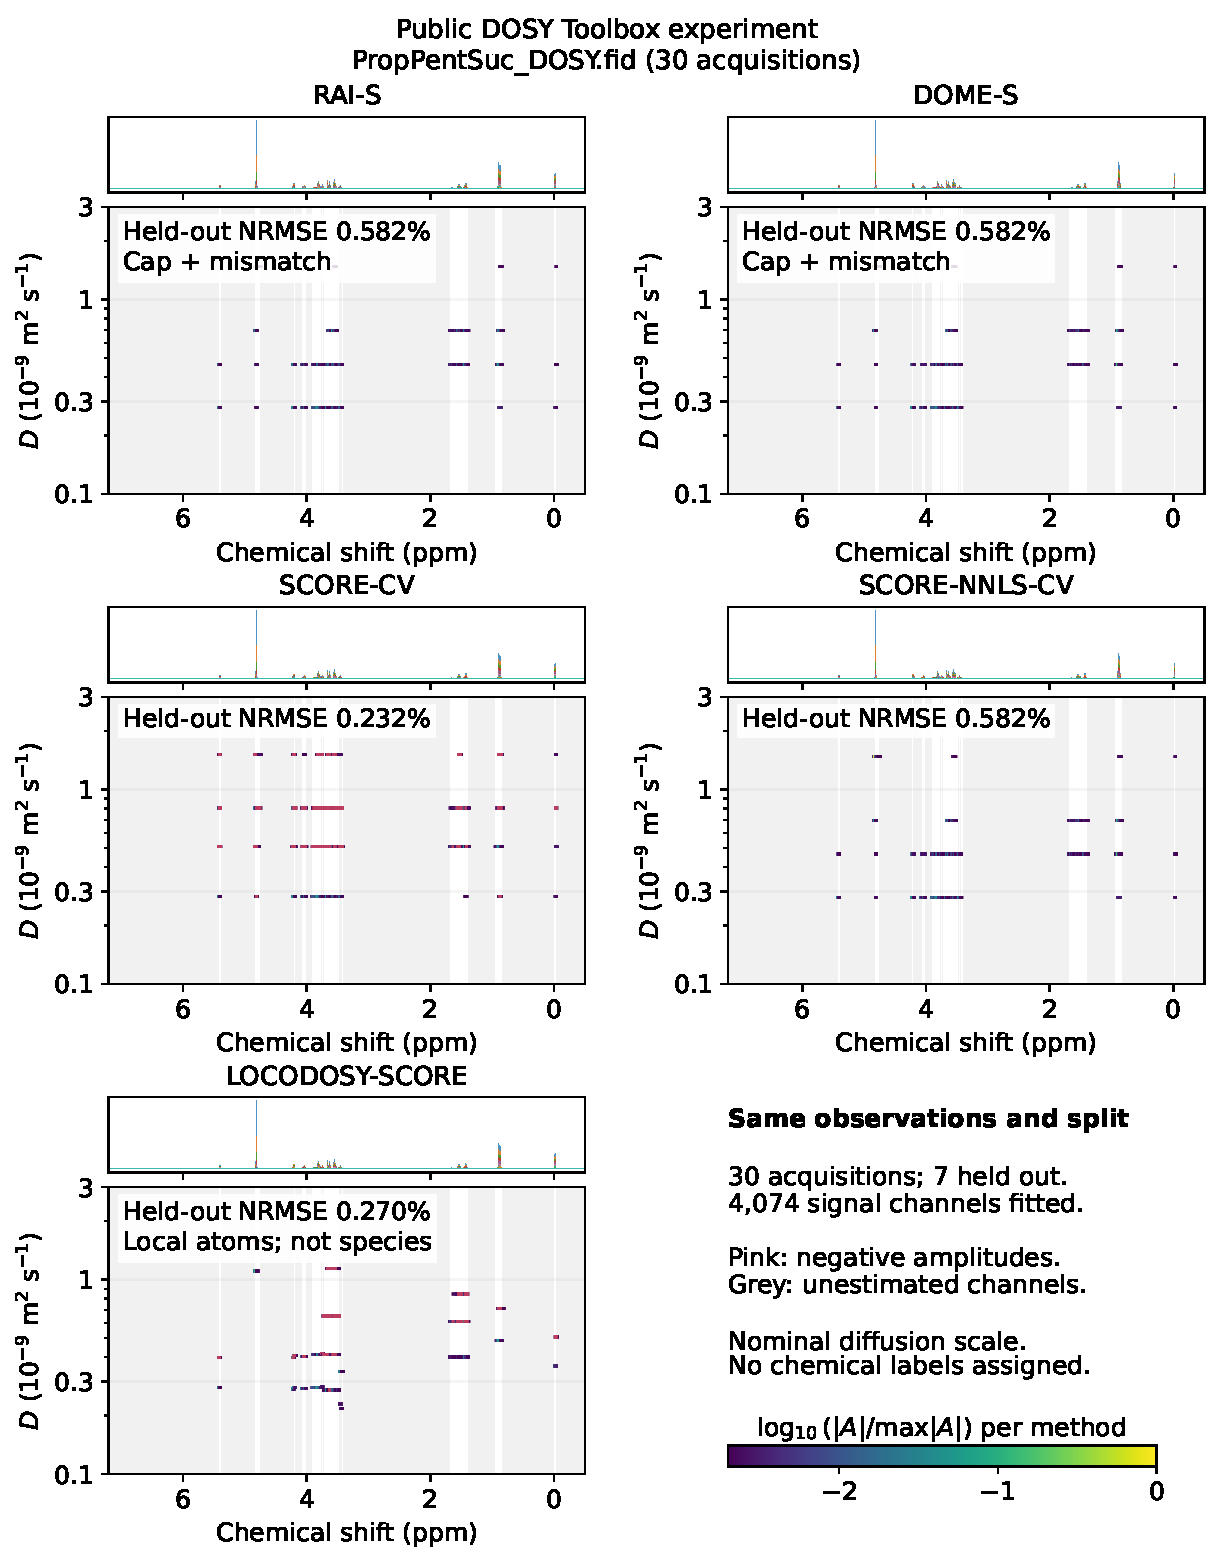
\includegraphics[width=\fulllength,height=0.86\textheight,keepaspectratio]{figures/public_mixture_comparison.pdf}
\caption{Public DOSY Toolbox example. Measured spectral families appear above
the training-only fitted atomic maps. Every selected spectral channel is fitted;
only the display of the upper traces is decimated. Pink denotes signed negative
amplitudes, grey denotes unestimated channels, and the 0.2\% relative display
cutoff does not prune the fit. Atomic rows have no inferred diffusion width or
assigned chemical identity.}
\label{fig:publicmixturerevision}
\end{adjustwidth}
\end{figure}

